\subsection{FREAK - Fast Retina Keypoint}

FREAK � um descritor bin�rio, composto por tr�s etapas:

\textbf{Amostragem de padr�o}

FREAK prop�e uma abordagem biol�gica para o reconhecimento de caracter�sticas, emulando o funcionamento
 da retina para amostragem de padr�o, como demonstrado na imagem \ref{fig:freak-sampler} que � um padr�o
  circular com maior densidade de pontos pr�ximo do centro, decrescendo
  exponencialmente.

\begin{figure}[H]
\centering
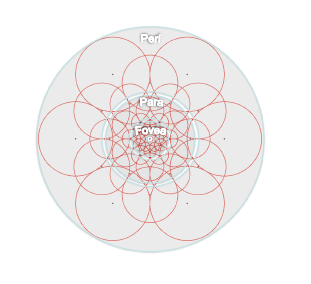
\includegraphics[scale=1.0]{images/freak-sampler}
\caption{Padr�o de amostradem do descritor FREAK}
\label{fig:freak-sampler}
\end{figure}


Cada amostra � suavizada com um kernel Gaussiano em que o raio do circulo ilustra o tamanho do desvio padr�o do kernel.
Como pode ser observado na figura~\ref{fig:freak-retina} o padr�o de amostragem corresponde com a distribui��o de receptores
 na retina.

\begin{figure}[H]
\centering
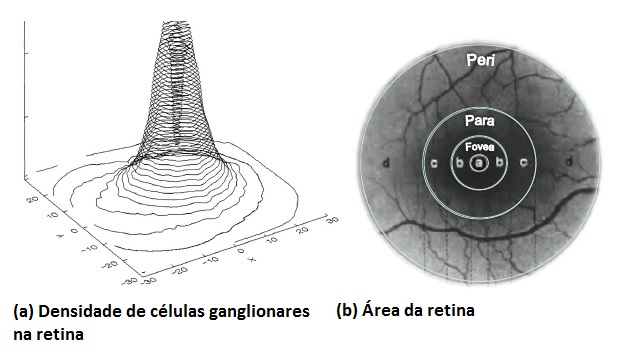
\includegraphics[scale=1.0]{images/freak-retina}
\caption{Distribui��o de receptores na retina}
\label{fig:freak-retina}
\end{figure}


\textbf{Compensa��o de Orienta��o}

Para estimar a rota��o dos \emph{keypoints}, s�o somados os gradientes locais
assim como no BRISK, entretanto ao inv�s de considerar os pontos de longa
dist�ncia, � considerado um padr�o de 45 pontos como mostrado na
figura~\ref{fig:freak-rotation}


\begin{figure}[H]
\centering
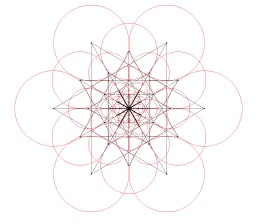
\includegraphics[scale=1.0]{images/freak-rotation}
\caption{Pares selecionados para calcular a orienta��o}
\label{fig:freak-rotation}
\end{figure}

Apesar de ter menos precis�o para recuperar informa��es de rota��o, como o n�mero de pontos 
� bem menor do que BRISK a quantidade de mem�ria armazenada � em geral 5 vezes menor.



\textbf{Compara��o de pares de amostragem}

Os pares de pontos s�o selecionados considerando a densidade maior no centro, 
como podemos observar na figura~\ref{fig:freak-retina} (a). 
Os pares come�am a ser comparados pelas extremidades e para dentro do centro, 
dessa forma otimizamos o reconhecimento pois com menos pontos podemos descartar casos em que 
a dist�ncia estiverem maiores do que um threshold, caso contr�rio prosseguimos para os outros 128 bits do descritor.


